%%%---%%%---%%%---%%%---%%%---%%%---%%%---%%%---%%%---%%%---%%%---%%%---%%%---%%%---%%%---%%%---%%%---%%%---%%%---%%%---%%%---%%%---%%%---%%%---%%%
%
\chapter{Technical background}
%
%%%---%%%---%%%---%%%---%%%---%%%---%%%---%%%---%%%---%%%---%%%---%%%---%%%---%%%---%%%---%%%---%%%---%%%---%%%---%%%---%%%---%%%---%%%---%%%---%%%
This chapter will present the important technical aspects involved in the developpement of the solution. Feel free to skip it and come back to it
as needed. (I will reference the different section at the relevant places throughout the text) (for this chapter, Im not sure if I should
have it or directly take its section and put them in the relevant places (i.e. put the IDE plugin section in the plugin chapter))

\begin{itemize}
	\item not sure if I shouldnt just discart this entire chapter because its not really relevant and the reader can find those information himself ?
	\item anyhow, clearly the less important chapter.
\end{itemize}

% 	%%%---%%%---%%%---%%%---%%%---%%%---%%%---%%%---%%%---%%%---%%%---%%%---%%%---%%%---%%%---%%%---%%%---%%%---%%%---%%%---%%%---%%%---%%%---%%%---%%%
% 	\section{Intellij IDE}
% 	%%%---%%%---%%%---%%%---%%%---%%%---%%%---%%%---%%%---%%%---%%%---%%%---%%%---%%%---%%%---%%%---%%%---%%%---%%%---%%%---%%%---%%%---%%%---%%%---%%%
% Not sure if talking about this is super relevant, but a big chunk of the thesis is about plugin developpement for intellij, 
% therefore it might be interesting to talk about it a bit ?
		%%%---%%%---%%%---%%%---%%%---%%%---%%%---%%%---%%%---%%%---%%%---%%%---%%%---%%%---%%%---%%%---%%%---%%%---%%%---%%%---%%%---%%%---%%%---%%%---%%%
		\subsection{Plugin developpement for Intellij IDE}
		%%%---%%%---%%%---%%%---%%%---%%%---%%%---%%%---%%%---%%%---%%%---%%%---%%%---%%%---%%%---%%%---%%%---%%%---%%%---%%%---%%%---%%%---%%%---%%%---%%%
Present briefly the structure of Intellij IDE and plugin structure, limitation and difficulties ? 

	%%%---%%%---%%%---%%%---%%%---%%%---%%%---%%%---%%%---%%%---%%%---%%%---%%%---%%%---%%%---%%%---%%%---%%%---%%%---%%%---%%%---%%%---%%%---%%%---%%%
	\section{Kotlin}
	%%%---%%%---%%%---%%%---%%%---%%%---%%%---%%%---%%%---%%%---%%%---%%%---%%%---%%%---%%%---%%%---%%%---%%%---%%%---%%%---%%%---%%%---%%%---%%%---%%%
	Might not be super relevant either, but since everything is made in kotlin,	maybe its interesting to at least mention it, and quickly highlight strenght of the language VS java ?

	%%%---%%%---%%%---%%%---%%%---%%%---%%%---%%%---%%%---%%%---%%%---%%%---%%%---%%%---%%%---%%%---%%%---%%%---%%%---%%%---%%%---%%%---%%%---%%%---%%%
	\section{TornadoFX framework}
	%%%---%%%---%%%---%%%---%%%---%%%---%%%---%%%---%%%---%%%---%%%---%%%---%%%---%%%---%%%---%%%---%%%---%%%---%%%---%%%---%%%---%%%---%%%---%%%---%%%
	High level presentation of important features - how it works and difference with javafx / swing ?

%%%---%%%---%%%---%%%---%%%---%%%---%%%---%%%---%%%---%%%---%%%---%%%---%%%---%%%---%%%---%%%---%%%---%%%---%%%---%%%---%%%---%%%---%%%---%%%---%%%
\chapter{Related work}
%%%---%%%---%%%---%%%---%%%---%%%---%%%---%%%---%%%---%%%---%%%---%%%---%%%---%%%---%%%---%%%---%%%---%%%---%%%---%%%---%%%---%%%---%%%---%%%---%%%

	% 6-12 pages (7- 14)
	% Discuter differente grammaire ?
	% parler de ce qui se fait en matière de parser et interface graphique



	% https://en.wikipedia.org/wiki/Parsing_expression_grammar


%%%---%%%---%%%---%%%---%%%---%%%---%%%---%%%---%%%---%%%---%%%---%%%---%%%---%%%---%%%---%%%---%%%---%%%---%%%---%%%---%%%---%%%---%%%---%%%---%%%
\section{The Moldable Debugger: a Framework for Developing Domain-Specific Debuggers}

%%%---%%%---%%%---%%%---%%%---%%%---%%%---%%%---%%%---%%%---%%%---%%%---%%%---%%%---%%%---%%%---%%%---%%%---%%%---%%%---%%%---%%%---%%%---%%%---%%%
\section{Antlr \cite{antlr}}

% \paragraph{} A translator maps each input sentence of a language to an output sentence.

% Recognition is much easier if you break it into two similar but distinct tasks or phases. The separate phases mirror how your brain reads English text. You don’t read a sentence character by character. Instead, you perceive a sentence as a stream of words. The human brain subconsciously groups character sequences into words and looks them up in a dictionary before recognizing grammatical structure. The first translation phase is called lexical analysis and operates on the incoming character stream. The second phase is called parsing and operates on a stream of vocabulary symbols, called tokens, emanating from the lexical analyzer. ANTLR automatically generates the lexical analyzer and parser for you by analyzing the grammar you provide.

% Performing a translation often means just embedding actions (code) within the grammar. ANTLR executes an action according to its position within the grammar. In this way, you can execute different code for different phrases (sentence fragments). For example, an action within, say, an expression rule is executed only when the parser is recognizing an expression.

% Some translations should be broken down into even more phases. Often the translation requires multiple passes, and in other cases, the translation is just a heck of a lot easier to code in multiple phases. Rather than reparse the input characters for each phase, it is more convenient to construct an intermediate form to pass between phases.

% This intermediate form is usually a tree data structure, called an ab- stract syntax tree (AST), and is a highly processed, condensed version of the input. Each phase collects more information or performs more computations. A final phase, called the emitter, ultimately emits output using all the data structures and computations from previous phases.

% Figure 1.1 illustrates the basic data flow of a translator that accepts characters and emits output. The lexical analyzer, or lexer, breaks up the input stream into tokens. The parser feeds off this token stream and tries to recognize the sentence structure. The simplest translators execute actions that immediately emit output, bypassing any further phases.

% \begin{figure}
% 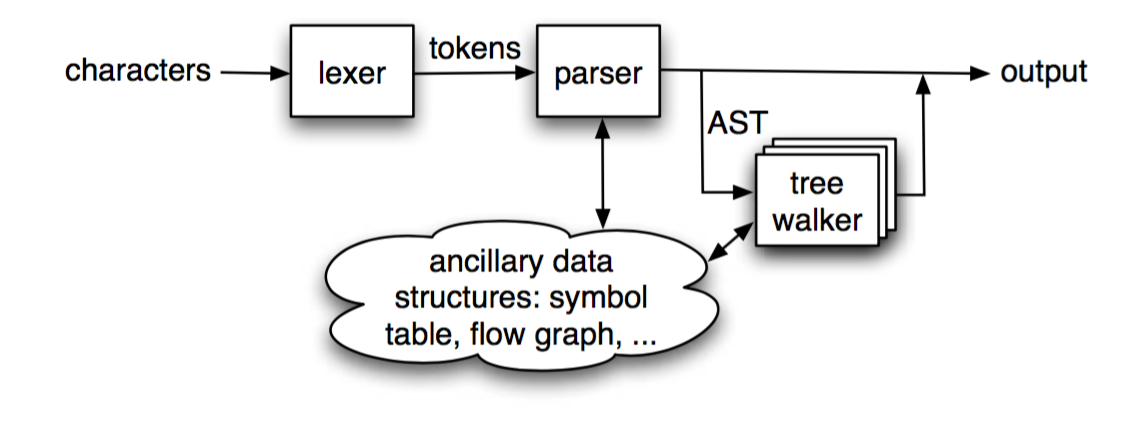
\includegraphics[width=\textwidth]{ressources/antlr1}
% \end{figure}

% \subsection{Nature of computer languages}
% Building translators with ANTLR requires you to use a formal language specification called a grammar. To understand grammars and to understand their capabilities and limitations, you need to learn about the nature of computer languages.
% The whole point of writing a grammar is so ANTLR can automatically build a program for you that recognizes sentences in that language. Unfortunately, starting the learning process with grammars and language recognition is difficult (from my own experience and from the questions I get from ANTLR users). The purpose of this chapter is to teach you first about language generation and then, at the very end, to describe language recognition. Your brain understands language generation very well, and recognition is the dual of generation. Once you understand language generation, learning about grammars and language recognition is straightforward. Here is the central question you must address concerning generation: how can you write a stream of words that transmits information beyond a simple list of items? In English, for example, how can a stream of words convey ideas about time, geometry, and why people don’t use turn signals? It all boils down to the fact that sentences are not just clever sequences of words, as Steven Pinker points out in The Lan- guage Instinct [Pin94]. The implicit structure of the sentence, not just the words and the sequence, imparts the meaning. What exactly is sen- tence structure? Unfortunately, the answer requires some background to answer properly. On the bright side, the search for a precise defini- tion unveils some important concepts, terminology, and language tech- nology along the way.

% \subsection{State machines}

% Is the lyrics state machine correct in the sense it generates valid blues sentences and only valid sentences? Unfortunately, no. The machine can also generate invalid sentences, such as “Your truck is sad and sad.” Rather than choose words (transitions) at random in each state, you could use known probabilities for how often words follow one an- other. That would help, but no matter how good your statistics were, the machine could still generate an invalid sentence. Apparently, human brains do something more sophisticated than this simple state machine approach to generate sentences. State machines generate invalid sentences for the following reasons: 

% Grammatical does not imply sensible. For example, “Dogs revert vacuum bags” is grammatically OK but doesn’t make any sense. In English, this is self-evident. In a computer program, you also know that a syntactically valid assignment such as employeeName= milesPerGallon; might make no sense. The variable types and meaning could be a problem. The meaning of a sentence is referred to as the semantics. The next two characteristics are related to syntax.

% There are dependencies between the words of a sentence. When confronted with a ], every programmer in the world has an involuntary response to look for the opening [.

% There are order requirements between the words of a sentence. You immediately see “(a[i+3)]” as invalid because you expect the ] and ) to be in a particular order (I even found it hard to type).

% So, walking the states of a state machine is too simple an approach for the generation of complex language. There are word dependencies and order requirements among the output words that it cannot satisfy. For- mally, we say that state machines can generate only the class of regular languages. As this section points out, programming languages fall into a more complicated, demanding class, the context-free languages. The difference between the regular and context-free languages is the differ- ence between a state machine and the more sophisticated machines in the next section. The essential weakness of a state machine is that it has no memory of what it generated in the past. What do we need to remember in order to generate complex language?

% To reveal the memory system necessary to generate complex language, consider how you would write a book. You don’t start by typing “the” or whatever the first word of the book is. You start with the concept of a book and then write an outline, which becomes the chapter list. Then you work on the sections within each chapter and finally start writ- ing the sentences of your paragraphs. The phrase that best describes the organization of a book is not “sequence of words.” Yes, you can read a book one word at a time, but the book is structured: chap- ters nested within the book, sections nested with the chapters, and paragraphs nested within the sections. Moreover, the substructures are ordered: chapter i must appear before chapter i+1. “Nested and ordered” screams tree structure. The components of a book are tree structured with “book” at the root, chapters at the second level, and so on.

% Interestingly, even individual sentences are tree structured. To demon- strate this, think about the way you write software. You start with a concept and then work your way down to words, albeit very quickly and unconsciously using a top-down approach. For example, how do you get your fingers to type statement x=0; into an editor? Your first thought is not to type x. You think “I need to reset x to 0” and then decide you need an assignment with x on the left and 0 on the right. You finally add the ; because you know all statements in Java end with ;. The image in Figure 2.2, on the following page, represents the implicit tree structure of the assignment statement. Such trees are called derivation trees when generating sentences and parse trees when recognizing sen- tences.

% It turns out that the humble stack is the perfect memory structure to solve both word dependency and order problems.4 Adding a stack to a state machine turns it into a pushdown machine (pushdown automa- ton). A state machine is analogous to a stream of instructions trapped within a single method, unable to make method calls. A pushdown machine, on the other hand, is free to invoke other parts of the machine and return just like a method call. The stack allows you to partition a machine into submachines. These submachines map directly to the rules in a grammar.
% Representing pushdown machines requires a different visualization called a syntax diagram, which looks like a flowchart. There is a flow- chart-like submachine per phrase (tree structure subtree). Figure 2.4, illustrates the syntax diagram for the assignment statement sentence structure. The rectangular elements generate vocabulary symbols, and the rounded elements invoke the indicated submachine. Like a method call, the pushdown machine returns from a submachine invocation upon reaching the end of that submachine.

% This section demonstrated that pushdown machines generate syntacti- cally valid sentences. In other words, each sentence that the pushdown machine generates has a valid interpretation. The next section demon- strates that, unfortunately, some valid sentences have more than one interpretation.



% The expression 3+4*5 is not ambiguous to an adult human. It means multiply 4 by 5 and add 3, yielding 23. An elementary school student doing the operations from left to right might ask, “Why is the result not 35?” Indeed, why not? Because mathematicians have decreed it so. In fact, German mathematician Leopold Kronecker went so far as to say, “God made the natural numbers; all else is the work of man.” So, the language is ambiguous, but syntax and some precedence rules make it unambiguous.

% Within a syntax diagram, an ambiguous sentence or phase is one that the diagram can generate following more than one path. For example, a syntax diagram for C can generate statement i*j; following the path for both a multiplicative expression and a variable definition (in other words, j is a pointer to type i). To learn more about the relationship of ambiguous languages to ANTLR grammars, see Section 11.5, Ambi- guities and Nondeterminisms, on page 273. For example, Section 11.5, Arithmetic Expression Grammars, on page 275 has an in-depth discus- sion of the arithmetic expression ambiguity.

% Although syntax is sometimes insufficient to interpret sentences, the informal language definition usually has some extra rules such as pre- cedence that disambiguate the sentences. Chapter 13, Semantic Predi- cates, on page 317 illustrates how to use semantic predicates to enforce these nonsyntactic rules. Semantic predicates are boolean expressions, evaluated at runtime, that guide recognition.

% \subsubsection{vocabulary symbols}
% Just as sentences consist of phrases, vocabulary symbols have struc- ture. In English, for example, a linguist sees the word destabilize as “de.stabil.ize.”7 Similarly, the real number 92.5 is two integers sepa- rated by a dot. Humans unconsciously scan sentences with these char- acters and group them into words.
% Sentences are actually sequences of characters, but your brain sees them as sequences of words as if they were complete symbols like Chi- nese characters. This happens no matter how long the words are. For example, the word for the Hawaiian state fish (Humuhumunukunukua- pua’a) is pretty long, but you read it as one symbol (pronouncing it is a lot harder). Your brain somehow implicitly forms words from the char- acters and looks them up in a dictionary of sorts.

% To mimic the technique your brain uses to recognize sentences, you need to separate the language-level processing from the vocabulary- level processing into two complete recognizers. The language-level rec- ognizer is usually called the parser, and the vocabulary recognizer is usually called the scanner, lexical analyzer, or lexer. Lexers create tokens9 (vocabulary symbols) and pass them to the parser. The only difference between the two recognizers is that the parser recognizes grammatical structure in a stream of tokens while the lexer recognizes structure in a stream of characters. Both perform essentially the same task, and ANTLR implements both using the same strategy.

% Separating the parser and lexer might seem like an unnecessary com- plication if you’re used to building recognizers by hand; however, the separation reduces what you have to worry about at each language level. You also get several implementation advantages: 

% The parser can treat arbitrarily long character sequences as sin- gle tokens. Further, the lexer can group related tokens into token “classes” or token types such as INT (integers), ID (identifiers), FLOAT (floating-point numbers), and so on. The lexer groups vocabulary symbols into types when the parser doesn’t care about the indi- vidual symbols, just the type. For example, the parser doesn’t care which integer is approaching on the input stream, just that it is an integer. Also, the parser does not have to wonder whether the next vocabulary symbol is an integer or floating-point number. The lexer can figure this out beforehand and send token type INT or FLOAT accordingly, allowing the parser to be much simpler.


% The parser sees a pipeline of tokens, which isolates it from the token source. The source of the tokens is irrelevant. For efficiency reasons, you want to save the results of lexing a character stream in a number of situations. For example, interpreters walk the same program statements multiple times during a loop. Once your lexer has tokenized the input, the parser can walk the same token buffer over and over. Some compilers (C and C++ come to mind) can even save tokenized header files to avoid repeatedly tokenizing them.

% The lexer can filter the input, sending only tokens of interest to the parser. This feature makes it easy to handle whitespace, com- ments, and other lexical structures that you want to discard. For example, if comments were passed to the parser, the parser would have to constantly check for comment tokens and filter them out. Instead, the lexer can simply throw them out, as shown in Fig- ure 2.7, on the previous page, or pass them to the parser on a hidden channel, as shown in Figure 2.8. The tokens on the hid- den channel are marked with an “x.” Note that the channel is an integer and you can put tokens on any channel you want, but the parser listens to only one channel. For more information about token channels, see Section 4.3, Lexical Rules, on page 107 and classes Token, CommonToken, and CommonTokenStream in the org.antlr.runtime package.

% At this point, you have the entire language generation picture. Sen- tences are not ingenious word sequences. Complex language generation enforces word dependencies and order requirements. Your brain enforces these constraints by subconsciously creating a tree structure. It does not generate sentences by thinking about the first word, the second word, and so on, like a simple state machine. It starts with the overall sentence concept, the root of the tree structure. From there the brain creates phrases and subphrases until it reaches the leaves of the tree structure. From a computer scientist’s point of view, generating a sentence is a matter of performing a depth-first tree walk and “saying” the words represented by the leaves. The implicit tree structure conveys the meaning.
% Sentence recognition occurs in reverse. Your eyes see a simple list of words, but your brain subconsciously conjures up the implicit tree structure used by the person who generated the sentence. Now you see why language recognition is the dual of language generation. ANTLR builds recognizers that mimic how your brain recognizes sentences. The next section gives you an intuitive feel for what sentence recog- nition by computer means. Afterward, you will be in good shape for Chapter 4, ANTLR Grammars, on page 86.

% The ANTLR parser generator accepting a larger class of grammars than LL(k) and generating recursive-descent parsers that are very similar to what a programmer would build by hand. 

\begin{itemize}
	\item ANTLR parser generator accepts a larger class of grammars than LL(k)
\end{itemize}
% \paragraph{SYNTAX DIAGRAM AND LOOKAHEAD DFA VISUALIZATION}
% 		ANTLR is a recursive-descent parser generator that accepts a large class of grammars called LL(*) that can be augmented with semantic and syntactic predicates 
% 		\subparagraph{LL($*$) and Lookahead DFA}
% 		ANTLR’s core parsing strategy is called LL(*) and is a natural extension to LL(k). LL(k) parsers make parsing decisions (i.e., distinguishing between alternative productions) using at most k symbols of lookahead. In contrast, LL(*) parsers can scan arbitrarily far ahead. Because LL(k) lookahead is bounded, the lookahead language is regular and can be encoded within an acyclic deterministic finite automaton (DFA) [6]. LL(*) simply allows cycles in the lookahead DFA. Lookahead decisions for LL(*) are no different than LL(k) decisions in that, once an alternative is predicted, LL parsing of that alternative proceeds normally.

% 		LL(*) represents a much larger class of grammars than LL(k) because parsing decisions can see past arbitrarily-long common left-prefixes. 

% 		A better solution is to recognize that, while this lookahead language is infinite, it is still regular and so there must be a (cyclic) DFA that recognizes sentences in that lookahead language. ANTLR automatically creates these lookahead DFA and makes them available to ANTLRWorks. Figure 1 is an ANTLRWorks screen shot showing a portion of the grammar as well as the lookahead DFA for the parsing decision in rule def. Being able to examine the lookahead DFA for a particular decision is very helpful when debugging grammars. Often it is not clear why a rule parses a certain input sequence improperly. Tracing that input sequence through the lookahead DFA reveals where it splits off down the wrong path, ultimately predicting the wrong alternative (currently ANTLRWorks does not visually step through the lookahead DFA).

% 		ANTLR’s use of a lookahead DFA at a decision point avoids the need for the full parser to backtrack. Running this DFA is much more efficient than running the general recursive-descent parsing process for each alternative for several reasons. First, the DFA lookahead process stops as soon as it reaches a point at which it can decide between the alternatives, and therefore it usually only looks at the first few tokens, even in a large recursive grammar rule. Second, the DFA lookahead process does not execute grammar actions, so there is no danger of executing them more than once or having to undo them.

% 		LL(*) does not approximate the distinguishing lookahead language nor the entire context-free grammar. A grammar is only LL(*) when the lookahead needed to distinguish alternative produc- tions is regular for each decision. This does not mean that the language generated by the grammar itself must be regular, however. The language generated by the following LL(1) rule is not regular, but the lookahead language used to distinguish productions is regular (’(’ or INT):

% 		\begin{verbatim}
% 	e : ’(’ e ’)’ // ’(’ predicts this alternative
% 	  | INT       // INT predicts this alternative
% 	  ;
%   		\end{verbatim}

%   		Not all lookahead languages are regular. When the lookahead computation encounters recursion reachable by more than one alternative, for example, the analysis algorithm fails rather than ap- proximating the lookahead. In this case, ANTLR can still generate a parser that uses backtracking to distinguish the alternatives at run-time. In practice, this means that ANTLR can accept any non-left-recursive grammar without complaint.


	\subsection{Antlrworks}

\begin{itemize}
	\item development environment for ANTLR grammars - parser nondeterminism visualizer (syntax diagrams and a time-traveling)
	\item grammar-aware editor with refactoring and navigation features, 
	\item a grammar interpreter
	\item domain-specific grammar debugger. 
\end{itemize}
	

	% ANTLRWorks’ primary contributions are a parser nondeterminism visualizer based upon syntax diagrams and a time-traveling debugger that pays special attention to parser decision-making by visualizing lookahead usage and speculative parsing during backtracking.

	% compute and display the parse tree associated with a particular input sequence and start rule—all without requiring a complete grammar and without having to generate code, compile, and run the application incorporating the parser.

	% It can rewind and replay the parse multiple times by re-executing the events without having to restart the actual parser. (my solution doesnt actually do time travel but provides as relevant information by being able to regenerate a state for a given parser and analyze the state of the system at the time of its execution)

	% The debugger dynamically displays a parser’s input stream, parse tree, generated abstract syntax tree (AST), rule invocation stack, and event stream as the user traces through the parser execution. The grammar, input, and tree display panes are always kept in sync so that clicking on, for example, an AST node shows the grammar element that created it and the token within the input stream from which it was created. ANTLRWorks has breakpoints and single-step facilities that allow programmers to stop the parser when it reaches a grammar location of interest or even an input phrase of interest. Sometimes it is useful to jump to a particular event (such as a syntax error) within the parse and then back up to examine the state of the parser before that event. To accommodate this, ANTLRWorks has a “step backwards” facility.

	% Complex language problems are often broken down into multiple phases with the first phase parsing the input and building an intermediate-form AST. This AST is then passed between multiple tree walkers to glean information or modify the AST. ANTLR accepts tree grammars and can automatically generate tree walkers, again in the form of a recursive-descent parser. The ANTLRworks debugger graphically illustrates the node-by-node construction of ASTs as the parser being debugged constructs these nodes. ASTs grow and shrink as the developer steps forward and backwards in the parse. ANTLR treats tree grammars just like parser grammars except that the input is a tree instead of a flat token sequence. In the ANTLRWorks debugger, programmers can set breakpoints in the input tree and single step through tree grammars to detect errors just like when debugging a token stream parser.

	
	% \subparagraph{Semantic Predicates}
	% Most programming languages are context-sensitive even though we describe them with context-free grammars for parsing efficiency reasons. Context-sensitive constructs are resolved with semantic actions during or after parsing to verify semantic validity. For example, “x=y;” only makes sense in the context of a visible variable declaration for y (and x in languages that require variables to be declared before use). In this case, context affects the validity, but not the meaning of the phrase. Syntax alone is sufficient to determine that the phrase is an assignment statement.

	% Inescapable context-sensitivity occurs when the proper interpretation of a phrase relies on in- formation about the surrounding context. Because there is no way to specify context in a pure context-free grammar, context-sensitivity results in ambiguous grammars. Ambiguous grammars can generate the same phrase in more than one way because the alternative productions cannot be predicated upon context. An ambiguous context-free grammar then has no deterministic parser (a parser that chooses exactly one phrase interpretation), rendering deterministic parsing tools based on pure context-free grammars ineffective in this case.

	% ANTLR augments context-free grammars with semantic predicates that can specify the semantic validity of applying a production, thus, providing a context-sensitive parsing mechanism. ANTLR is applicable to languages such as C++ that present a number of challenging parsing problems. One of the most difficult issues involves a syntactic ambiguity that must be resolved with symbol table information. Consider phrase C++ expression “T(34)”. This phrase can be either a constructor style typecast or a method call depending on whether T is a type name or a method name.

	% \subparagraph{Syntactic Predicates and Backtracking}
	% One weakness of the LL(*) approach is that a DFA does not have a stack and consequently cannot see past nested language structures; that is, LL(*) cannot see past recursive rule invocations to what lies beyond. To overcome this limitation, ANTLR supports syntactic predicates that predicate alter- native productions with a context-free lookahead language rather than the weaker regular lookahead language used by LL(*). Syntactic predicates not only increase the strength of LL(*) by providing a controlled backtracking mechanism, but they also provide a means of resolving grammar ambiguities.

	\paragraph{RAPID PROTOTYPING - time travel}

	
	My solution doesnt actually do time travel but provides as relevant information by being able to regenerate a state for a given parser and analyze the state of the system at the time of its execution

	% In order to develop a correct grammar quickly, the developer needs the ability to test rules as they are written. As the grammar grows, the developer adds rules to an existing base of tested rules, making it easier to track down parse errors (the errors are most likely in any newly added rules). The developer needs more than just a yes or no answer as to whether or not the input sequences match—they need parse trees, which describe exactly how the grammar matched the input sequences. Ideally, this testing would be done without code generation and target-language compilation in order to provide instantaneous feedback.

	% ANTLRWorks supports rapid grammar development by using ANTLR’s built-in interpreter, thus, providing immediate feedback during development (Meta-Environment [11] [19], TextTransformer [20], and LAUNCHPADS [21] also have interpreters).

% 	\paragraph{GRAMMAR DEBUGGER}
% 	Completing a grammar project involves verifying that the resulting parser matches input correctly, detects erroneous input, and builds a proper data structure or emits proper output. By single stepping and using breakpoints, a debugger helps clear up grammar issues but more importantly highlights which user actions are executed and in what order. Tracing through a grammar also helps track down errors in tree construction.

% 	While all of this can be accomplished clumsily using a generic programming language debugger, generic debuggers offer little more than stepping through methods and evaluating raw expressions. ANTLRWorks’ debugger, on the other hand, focuses on the higher level, domain-specific data struc- tures and processes associated with language recognition. ANTLRWorks displays input streams, parser lookahead, parse trees, parse stacks, and ASTs as they change during recognition and ensures that all visualizations stay in sync.
% 		\subparagraph{Parse Tree Visualization}
% 		\subparagraph{Debugging syntactic predicates}
% 		\subparagraph{Socket Protocol, Debug Events, and Language-Independent Debug- ging}
% 		\subparagraph{Breakpoints and Single Stepping}
% 		\subparagraph{Rewind and Stepping Backwards}
% 		When tracking down parse errors or problems related to improperly recognized input sequences, often the most crucial piece of information is what happens right before an error occurs or the parser recognizes a particular input sequence.
% 		\subparagraph{AST Visualization}

% Translators are often broken into multiple phases out of necessity because of symbol resolution issues or purely for simplicity reasons. The first phase is a parser that builds ASTs (and possibly other data structures such as a symbol table). When the grammar produces an incorrect AST, it can be difficult to track down exactly where in the grammar the erroneous subtree is created. ANTLRWorks visually displays ASTs as they are built so that the developer can single step through the grammar at the appropriate input position to discover why the improper tree is being created. The developer can view trees as two-dimensional graphs or as hierarchal lists, which are sometimes easier to visualize for very large inputs. Finally, as with the parse trees, ANTLRWorks shows the relationship between AST nodes, the input stream, and the grammar.
% 		\subparagraph{Debugging Tree Parsers}
% 		\subparagraph{related word}
% 		There are numerous tools related to grammar development environments with graphical interfaces. Most of them are academic, but there are some commercial tools. Some of the academic tools are focused on generating language development editors or other applications using generative pro- gramming from syntax and semantic specifications. ANTLRWorks is tightly focused on grammar development itself rather than grammar development as a means to creating another application. In that sense, ANTLRWorks has more in common with commercial tools, which are typically parser generators that come with grammar development environments.

% Every commercial grammar development tool has a debugger, but only ProGrammar and Text- Transformer have the data-centric breakpoint feature. ANTLRWorks has three main advantages: (1) its rewind and replay mode based on the event stream, (2) its ability to attach to a remote parser running on another machine, (3) its ability to debug parsers written in any language.

% There are a number of academic tools that allow you to develop grammars such as ASF+SDF’s Meta-Environment [11], LAUNCHPADS [21], Synthesizer Generator [30] (has now become com- mercial), SmartTools [31], LISA [32], and GTB [33] (Grammar ToolBox). Meta-Environment has grammar-aware editing, on-the-fly parser generation (supporting immediate grammar testing), GLR parse forest visualization, and some nice features that identify grammar issues such as useless sym- bols, typos, and inconsistent priorities and associativity. Meta-Environment can also generate syntax highlighters and debuggers for languages described by grammars, which includes debugging its own grammars [19]. ANTLRWorks’ debugger is less general because it works only on ANTLR grammars but is commensurately simpler and more task specific.


% LISA has a number of features that are similar to ANTLRWorks including a grammar-aware editor, BNF viewer, syntax tree viewer, and automata visualizer. Like Meta-Environment and Syn- thesizer Generator, LISA can automatically generate syntax directed editors and other visualization tools.
% While GTB has a variety of visualization views to show grammars, finite automata, and grammar dependency graphs, GTB is not strictly speaking an interactive grammar development environment. In the related world of natural language processing, Allman and Beale [34] provide a system for building natural language grammars using a visual interface and also contains a grammar debugger. DDF [35] (DSL Debugger Framework) is a set of Eclipse plugins for debugging domain specific languages described with ANTLR grammars. Aspects are used to weave in support code that maps the generated general purpose code back into the domain specific language source code. DDF reuses the existing Java Eclipse general debugger to debug domain specific languages. DDF is similar to ANTLR Studio in that both map generated code back to a domain specific language, (an ANTLR grammar in ANTLR Studio’s case and the domain specific language source code in DDF’s case). In
% contrast, ANTLRWorks uses a custom parser debugger that works with any target language. Finally, we understand that a grammar development environment for SableCC [36] is under
% construction.


%%%---%%%---%%%---%%%---%%%---%%%---%%%---%%%---%%%---%%%---%%%---%%%---%%%---%%%---%%%---%%%---%%%---%%%---%%%---%%%---%%%---%%%---%%%---%%%---%%%
\section{Ohm}
%%%---%%%---%%%---%%%---%%%---%%%---%%%---%%%---%%%---%%%---%%%---%%%---%%%---%%%---%%%---%%%---%%%---%%%---%%%---%%%---%%%---%%%---%%%---%%%---%%%